Bell numbers are a notion of combinatorics. It is \textbf{not} related to the famous Bell inequality in quantum physics. $B_n$ counts the number of partitions in a set $I$ of size $n$~\cite{knuth, OEIS-Bell}, i.e.\@~the number of sets of disjoint subsets of $I$ whose union is $I$. For example, $\{\{1, 2\}, \{3\}\}$ and $\{\{1, 2, 3\}\}$ are partitions of $I = \{1, 2, 3\}$.

Bell numbers are given by~\autoref{yoshi} which is due to Yoshisuke Matsunaga from the Japanese Edo era~\cite{knuth}.

\begin{theorem}[Yoshisuke Matsunaga] \label{yoshi}
    \begin{equation}
        B_{n+1} = \sum_{k=0}^n \binom{n}{k} B_k
    \end{equation}
\end{theorem}

For the purpose of analysing the complexity of the \texttt{truncated cumulants}(cf.\@~\ref{cumulant-method}), we need to estimate the asymptotic behavior of $B_n$. We use the result of de Bruijn~\cite{deBruijn}.


\begin{theorem}[De Bruijn]
    \begin{equation}
        \frac{\ln{B_n}}{n} = \ln{n} - \ln{\ln{n}} - 1 + o(1)
    \end{equation}
\end{theorem}

In a hand-waving approach, we could say that $B_n$ "behaves" as $n^n$, which signifies an exponential growth. Indeed, this can be seen in the plot~\autoref{fig:Capture_Bell} from~\cite{Graph-Bell}.

\begin{center}
    \begin{figure}[h!]
      \centering
      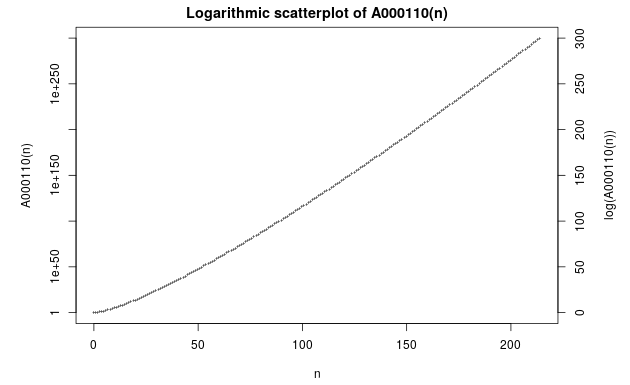
\includegraphics[width=0.6\linewidth]{Pics/Capture_Bell.PNG}
      \caption{Plot of Bell numbers from the OEIS \cite{Graph-Bell} in $\log_{10}$ scale}
      \label{fig:Capture_Bell}
    \end{figure}
\end{center}